\documentclass[12pt]{article}
\usepackage[a4paper, margin=0.75in]{geometry}
\usepackage[document]{ragged2e}
\usepackage{graphicx}
\usepackage{subcaption}
\usepackage{placeins}
\graphicspath{ {./images/} }
\usepackage{enumerate}
\usepackage{framed}
\usepackage{amsmath,amsfonts,amsthm,thmtools,amssymb,mathtools,commath}
\usepackage{physics}
\usepackage{tikz}
\usetikzlibrary{mindmap}
\usepackage{caption}
\usepackage{xcolor}
\usepackage[most]{tcolorbox}
\usepackage{cleveref}


%%%%%%%%%%%%%%%%
%  Definition  %
%%%%%%%%%%%%%%%%
\tcbuselibrary{theorems,skins,hooks}
\newtcbtheorem[number within=subsection]{definition}{Definition}%
{
    % theorem style=definition,
    enhanced,
	before skip=2mm,after skip=2mm, colback=cyan!5,colframe=cyan!80!black,boxrule=0.5mm,
	attach boxed title to top left={xshift=1cm,yshift*=1mm-\tcboxedtitleheight},
	boxed title style={frame code={
					\path[fill=cyan]
					([yshift=-1mm,xshift=-1mm]frame.north west)
					arc[start angle=0,end angle=180,radius=1mm]
					([yshift=-1mm,xshift=1mm]frame.north east)
					arc[start angle=180,end angle=0,radius=1mm];
					\path[left color=cyan!30!black,right color=cyan!30!black,
						middle color=cyan!50!black]
					([xshift=-2mm]frame.north west) -- ([xshift=2mm]frame.north east)
					[rounded corners=1mm]-- ([xshift=1mm,yshift=-1mm]frame.north east)
					-- (frame.south east) -- (frame.south west)
					-- ([xshift=-1mm,yshift=-1mm]frame.north west)
					[sharp corners]-- cycle;
				},interior engine=empty,
		},
	fonttitle=\bfseries,
	title={#2},#1
}{def}


%%%%%%%%%%%%%
%  Theorem  %
%%%%%%%%%%%%%
\tcbuselibrary{theorems,skins,hooks}
\newtcbtheorem[use counter from=definition]{theorem}{Theorem}%
{
    theorem style=plain,
    enhanced,
    colframe=green,
    boxrule=1pt,
    titlerule=0mm,
    toptitle=1mm,
    bottomtitle=1mm,
    fonttitle=\bfseries,
    fontupper=\mdseries\itshape,
    coltitle=green!30!black,
    colbacktitle=cyan!15!white,
    colback=green!10,
    description font=\bfseries\sffamily
}{thrm}


%%%%%%%%%%%%%%
% Corollary  %
%%%%%%%%%%%%%%
 \tcbuselibrary{theorems,skins}
 \newtcbtheorem[use counter from=theorem]{corollary}{Corollary}%
 {
    theorem style=plain,
    enhanced,
    colframe=green,
    frame hidden,
    titlerule=0mm,
    toptitle=1mm,
    bottomtitle=1mm,
    fonttitle=\bfseries,
    fontupper=\mdseries\itshape,
    coltitle=green!30!black,
    colbacktitle=cyan!15!white,
    colback=green!10,
    description font=\bfseries\sffamily
 }{corl}


%%%%%%%%%%%%%
%  Example  %
%%%%%%%%%%%%%
\tcbuselibrary{theorems,skins,hooks}
\newtcbtheorem[number within=section]{example}{Example}%
{
	enhanced,
	breakable,
	colback = gray!5,
	frame hidden,
	boxrule = 0sp,
	borderline west = {2pt}{0pt}{gray},
	sharp corners,
	detach title,
	before upper = \tcbtitle\par\smallskip,
    coltitle=gray!70!black,
	fonttitle = \bfseries\sffamily,
	description font = \mdseries\bfseries
}
{xmp}


%%%%%%%%%%%%%%
%  Exercise  %
%%%%%%%%%%%%%%
\tcbuselibrary{theorems,skins,hooks}
\newtcbtheorem[number within=section]{exercise}{Exercise}%
{
    enhanced,
    breakable,
    colback=black!5,
    colframe=black!30,
    left=0.5em,
    before skip=10pt,
    after skip=10pt,
    boxrule=0pt,
    boxsep=0pt,
    arc=0pt,
    outer arc=0pt,
    borderline west={3pt}{0pt}{black!30},
}{exc}

%%%%%%%%%%
%  Note  %
%%%%%%%%%%
\usetikzlibrary{arrows,calc,shadows.blur}
\tcbuselibrary{skins}
\newtcolorbox{note}[1][]{%
	enhanced jigsaw,
	colback=gray!20!white,%
	colframe=gray!80!black,
	size=small,
	boxrule=1pt,
	title=\textbf{Note:-},
	halign title=flush center,
	coltitle=black,
	breakable,
	drop shadow=black!50!white,
	attach boxed title to top left={xshift=1cm,yshift=-\tcboxedtitleheight/2,yshifttext=-\tcboxedtitleheight/2},
	minipage boxed title=1.5cm,
	boxed title style={%
			colback=white,
			size=fbox,
			boxrule=1pt,
			boxsep=2pt,
			underlay={%
					\coordinate (dotA) at ($(interior.west) + (-0.5pt,0)$);
					\coordinate (dotB) at ($(interior.east) + (0.5pt,0)$);
					\begin{scope}
						\clip (interior.north west) rectangle ([xshift=3ex]interior.east);
						\filldraw [white, blur shadow={shadow opacity=60, shadow yshift=-.75ex}, rounded corners=2pt] (interior.north west) rectangle (interior.south east);
					\end{scope}
					\begin{scope}[gray!80!black]
						\fill (dotA) circle (2pt);
						\fill (dotB) circle (2pt);
					\end{scope}
				},
		},
	#1,
}


\title{
    \textbf{\Large Experiment 5}\\
    \textbf{\Large Experiments on Class AB and Class C Amplifier}
}

\author{
    Turja Roy\\
    2108052
}
\date{February 20, 2024}

\begin{document}
\maketitle

\section{Objective}
\begin{enumerate}
    \item To study the working principle of a Class AB Amplifier.
    \item To study the working principle of a Class C Amplifier.
\end{enumerate}

\section{Apparatus}
\begin{enumerate}
    \item Transistors (2N3904 npn) - 2
    \item Resistors
    \item Capacitors
    \item DC Power Supply (0-30V)
    \item Function Generator
    \item Oscilloscope
    \item Multimeter
    \item Breadboard, Connecting wires, etc.
\end{enumerate}

\section{Circuit Diagram}
In the following page is given the circuit diagram for the Class AB Amplifier and Class C Amplifier. \\~\\

In Figure 1, The Class AB amplifier was built using two npn transistor. The input signal was given parallelly to the bases of the transistors. The transistor bases were connected by two diodes to overcome the crossover distortion. The emitter of $Q_1$ was connected to the collector of $Q_2$ and the output was taken from the collector of $Q_2$. The $100 \Omega$ resistor was used as the load resistor in the circuit. Oscilloscope has been connected in the shown way to get the input and output curves. \\~\\

In Figure 2, the Class C amplifier was built using a single npn transistor. The input signal was given to the base of the transistor. The output was taken from the emitter of the transistor. The $10 \; k\Omega$ resistor was used as the load resistor in the circuit. Oscilloscope has been connected in the shown way to get the input and output curves.

\begin{figure}[!htpb]
    \centering
    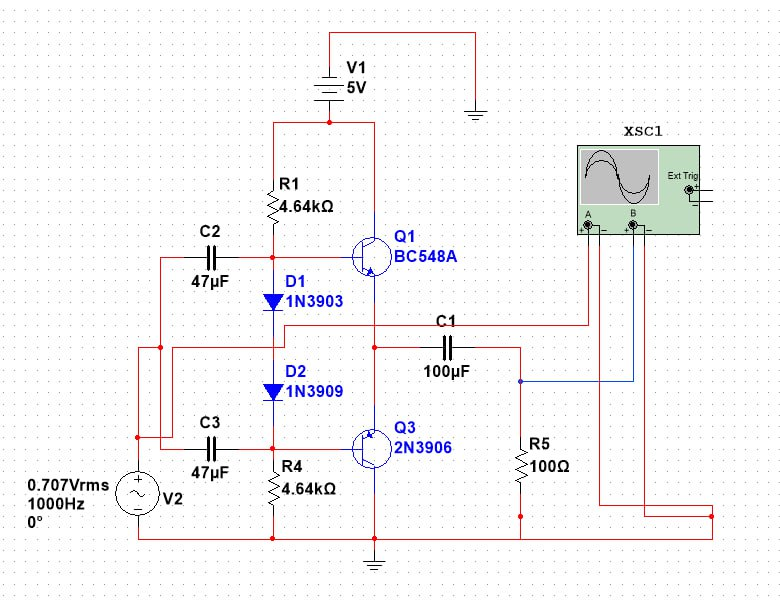
\includegraphics[width=0.8\textwidth]{Class_AB_Diagram.jpg}
    \caption{Class AB Amplifier Circuit Diagram}
\end{figure}

\begin{figure}[!htpb]
    \centering
    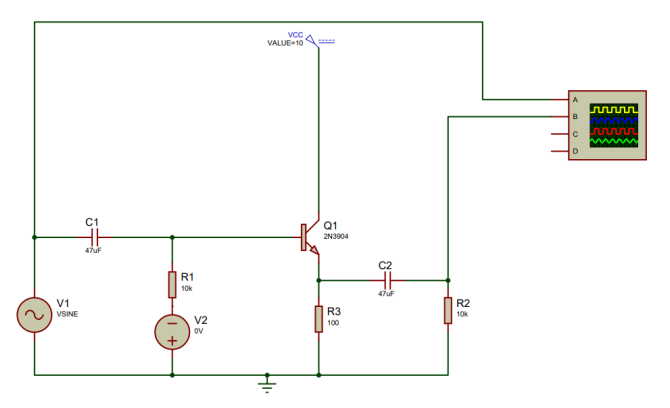
\includegraphics[width=0.8\textwidth]{Class_C_Diagram.png}
    \caption{Class C Amplifier Circuit Diagram}
\end{figure}

\FloatBarrier
\section{Result Analysis}

\subsection{Class AB Amplifier}
The Class AB amplifier is a combination of Class A and Class B amplifier. The input signal is divided into two halves and each half is amplified by one transistor. The bases of the transistors are connected by two diodes to overcome the crossover distortion. The output of these two transistors are then combined to get the amplified output.

\subsubsection{Class AB Amplifier Input and Output Graphs}

\begin{figure}[h!]
    \centering
    \begin{subfigure}{0.55\textwidth}
        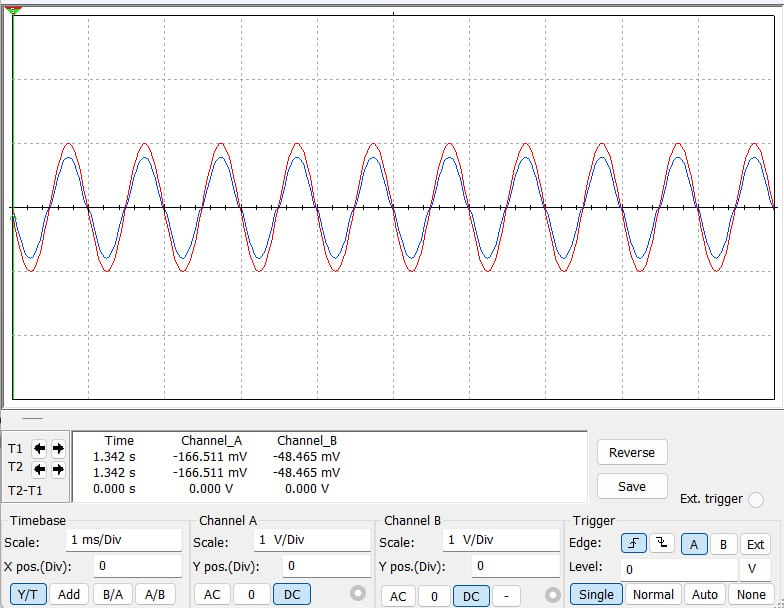
\includegraphics[width=\textwidth]{Class_AB_Graph.jpg}
        \caption{Simulated Graph}
    \end{subfigure}
    \begin{subfigure}{0.55\textwidth}
        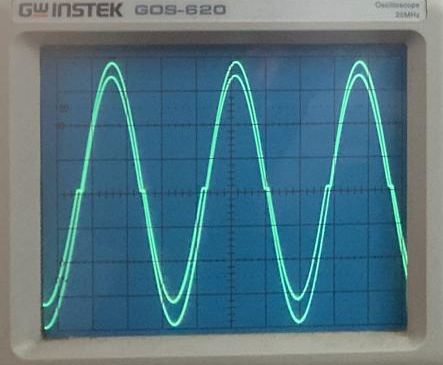
\includegraphics[width=\textwidth]{Class_AB_Practical.png}
        \caption{Experimental Graph}
    \end{subfigure}
    \caption{Simulated and Practical Input and Output Graphs for Class AB Amplifier}
\end{figure}

In the simulated graph (Figure 3-a), the red and the blue lines show the input and output curves respectively. In the practical graph (Figure 3-b), we see that the crossover distortion is almost negligible. The output curve is almost similar to the input curve.

\subsection{Class C Amplifier}
The Class C amplifier is a type of amplifier where the transistor conducts for less than half of the input cycle. The input signal is given to the base of the transistor and the output is taken from the emitter of the transistor. The transistor conducts only when the input signal is greater than the base-emitter voltage of the transistor.

\subsubsection{Class C Amplifier Input and Output Graphs}

\begin{figure}[h!]
    \centering
    \begin{subfigure}{0.55\textwidth}
        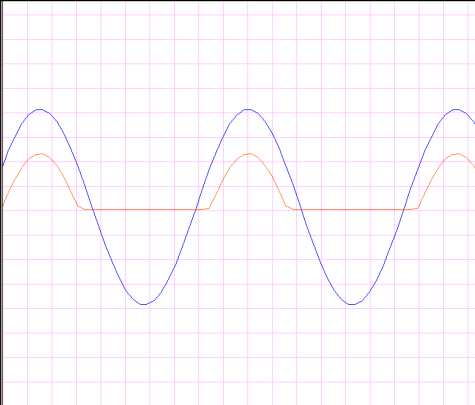
\includegraphics[width=\textwidth]{Class_C_Graph.png}
        \caption{Simulated Graph}
    \end{subfigure}
    \begin{subfigure}{0.55\textwidth}
        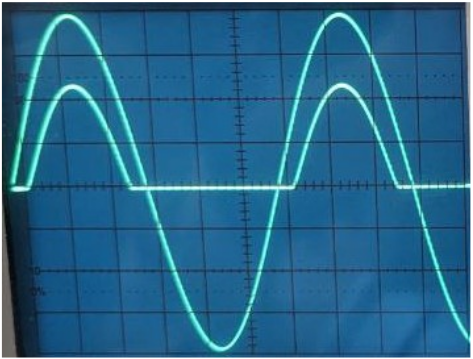
\includegraphics[width=\textwidth]{Class_C_Practical.png}
        \caption{Experimental Graph}
    \end{subfigure}
    \caption{Simulated and Practical Input and Output Graphs for Class AB Amplifier}
\end{figure}

In the simulated graph (Figure 4-a), the blue and the red lines show the input and output curves respectively. In the practical graph (Figure 4-b), we see that the input and output curves are almost similar to that of the simulated graph.

\FloatBarrier
\section{Discussion}
The experiment was conducted to observe the amplification of a signal in Class AB amplifier and Class C amplifier. In the Class C amplifier, the Q-point is set below the cutoff region. The transistor conducts only when the input signal is greater than the base-emitter voltage of the transistor. \\~\\

In the Class AB amplifier, the Q-point is set at the cutoff region. To overcome the crossover distortion, the bases of the transistors are connected by two diodes. In the experiment, it was observed that the output curve was almost similar to the input curve, and the crossover distortion was almost negligible.

\end{document}
